\section{Electronics and readout}

\F{electronicScheme} shows a schematic diagram of the electronics and readout used for the Cherenkov detector.

The XP4500B Photonis photomultipliers are powered in positive polarity by a CAEN SY4527 outfitted with 1501P boards.

There are two anode signals from the tubes. One of them is connected directly to Flash ADC
boards built at Jefferson Lab, the Flash ADC module FADC250. The FADC250 sampling frequency is $250 MHz$. The other signals is discriminated by a DSC2 unit and connected to CAEN v1190 TDC modules.
The TDCs were set to have 50ps/channel timing resolution.

The Cherenkov FADC250 and TDC information is read out using the CEBAF Online Data Acquisition system (CODA).

\begin{figure}
	\centering
	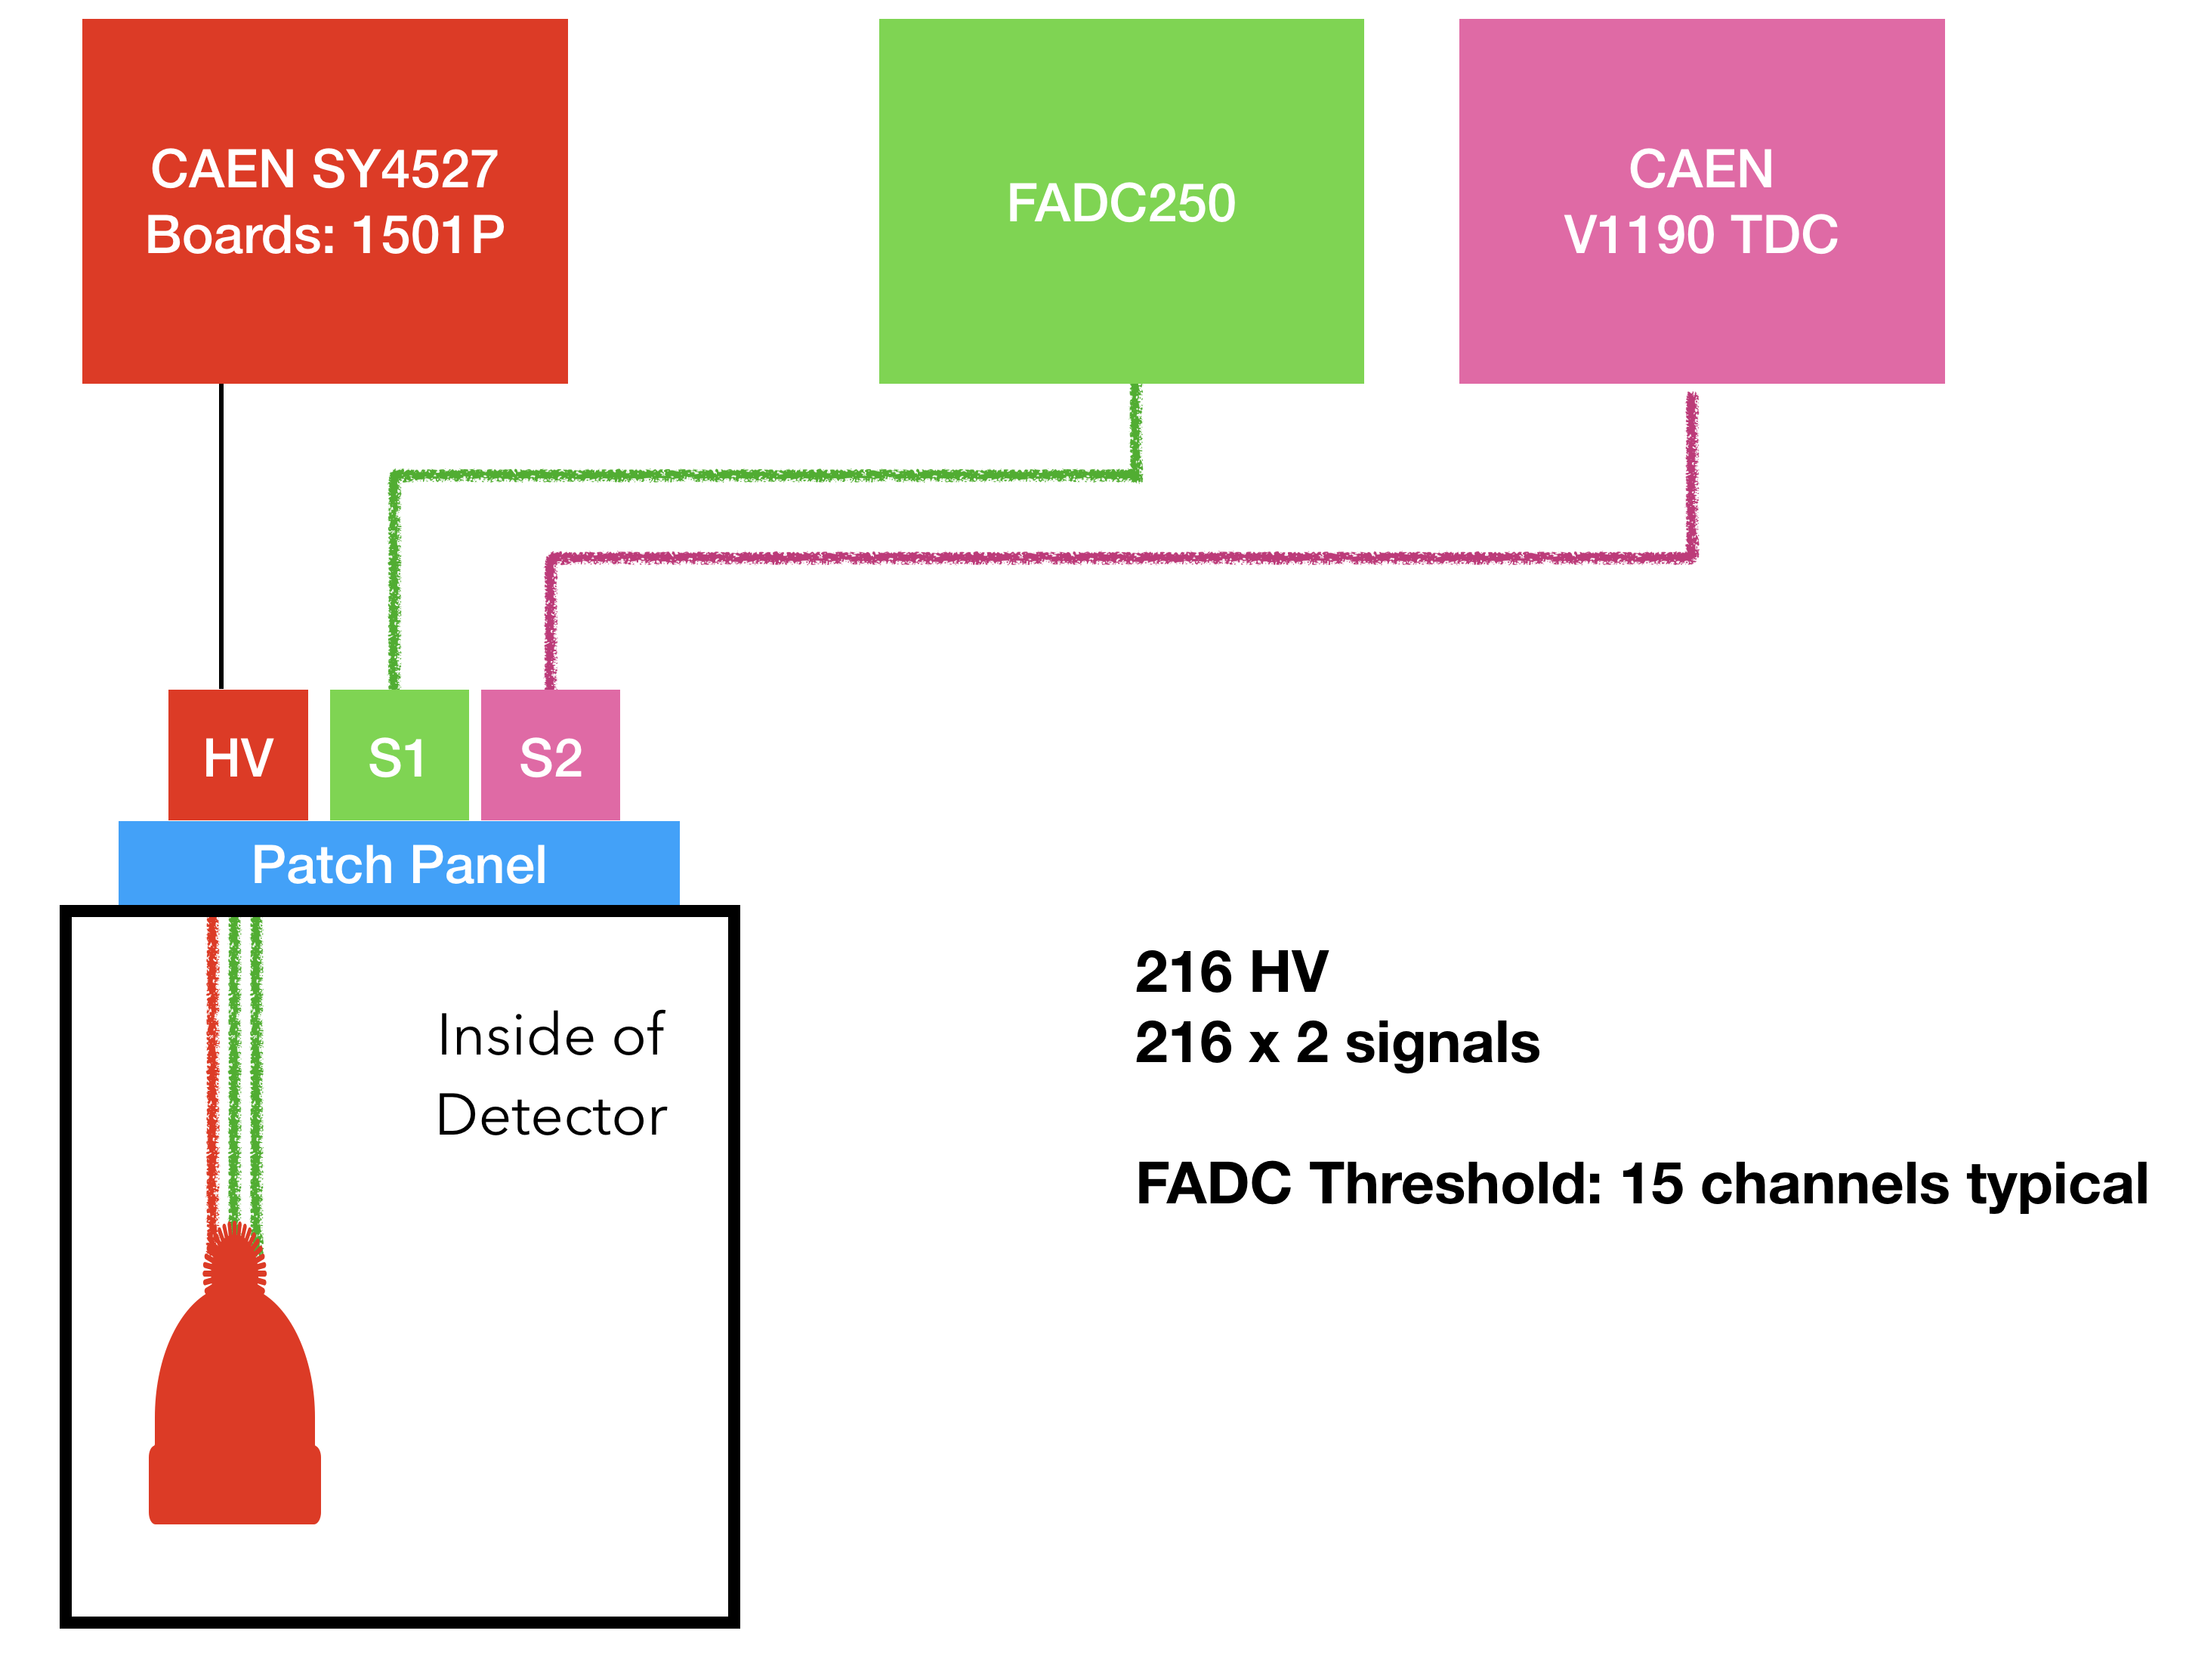
\includegraphics[width=0.95\columnwidth,keepaspectratio]{img/electronicScheme.png}
	\caption{The electronic schematic of the LTCC.}
	\label{fig:electronicScheme}
\end{figure}





A typical signal from the FADC250 module is shown in \F{fadc}. The signal is usually contained in 3 to 5 time samples (each time sample is 4 ns).
In order to be written to tape, at least one of the 100 signals must be above a 30 channels threshold. The FADC250 then consider a time window 16 ns (4 samples)
before the threshold crossing time, for the duration of 20 samples (80 ns). The final integrated charge used in the reconstruction code is the signal integral
minus the electronic pedestal, as described in \F{fadc}.



\begin{figure}
	\centering
	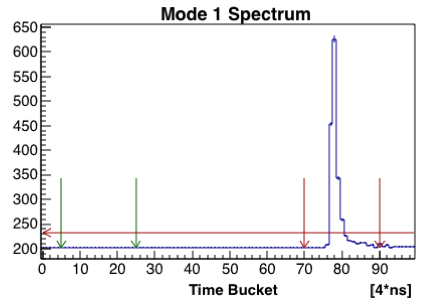
\includegraphics[width=0.95\columnwidth,keepaspectratio]{img/fadc.png}
	\caption{The FADC250 digitized output as a function of sample index of one of the LTCC PMT, self triggering on the single photo-electron signal.
            The CODA system saves a 400 ns time window (100 samples) if at least one of the 100 signals is above a 30 channels threshold.
				The integral signal is the sum of the output at the sample indexes between the two red arrows:
            the left red arrow is placed 4 samples before the signal crosses the threshold,
            and the right red arrow is 20 samples after that. The final integrated charge used in the reconstruction code is this integral minus the pedestal.
            The pedestal is calculated using the average of the signal between the green arrows.
				The absolute position of the peak and green arrows, and the relative position of the red arrows are adjusted in CODA parameters loaded before each run.}
	\label{fig:fadc}
\end{figure}




%\begin{figure}
%	\centering
%	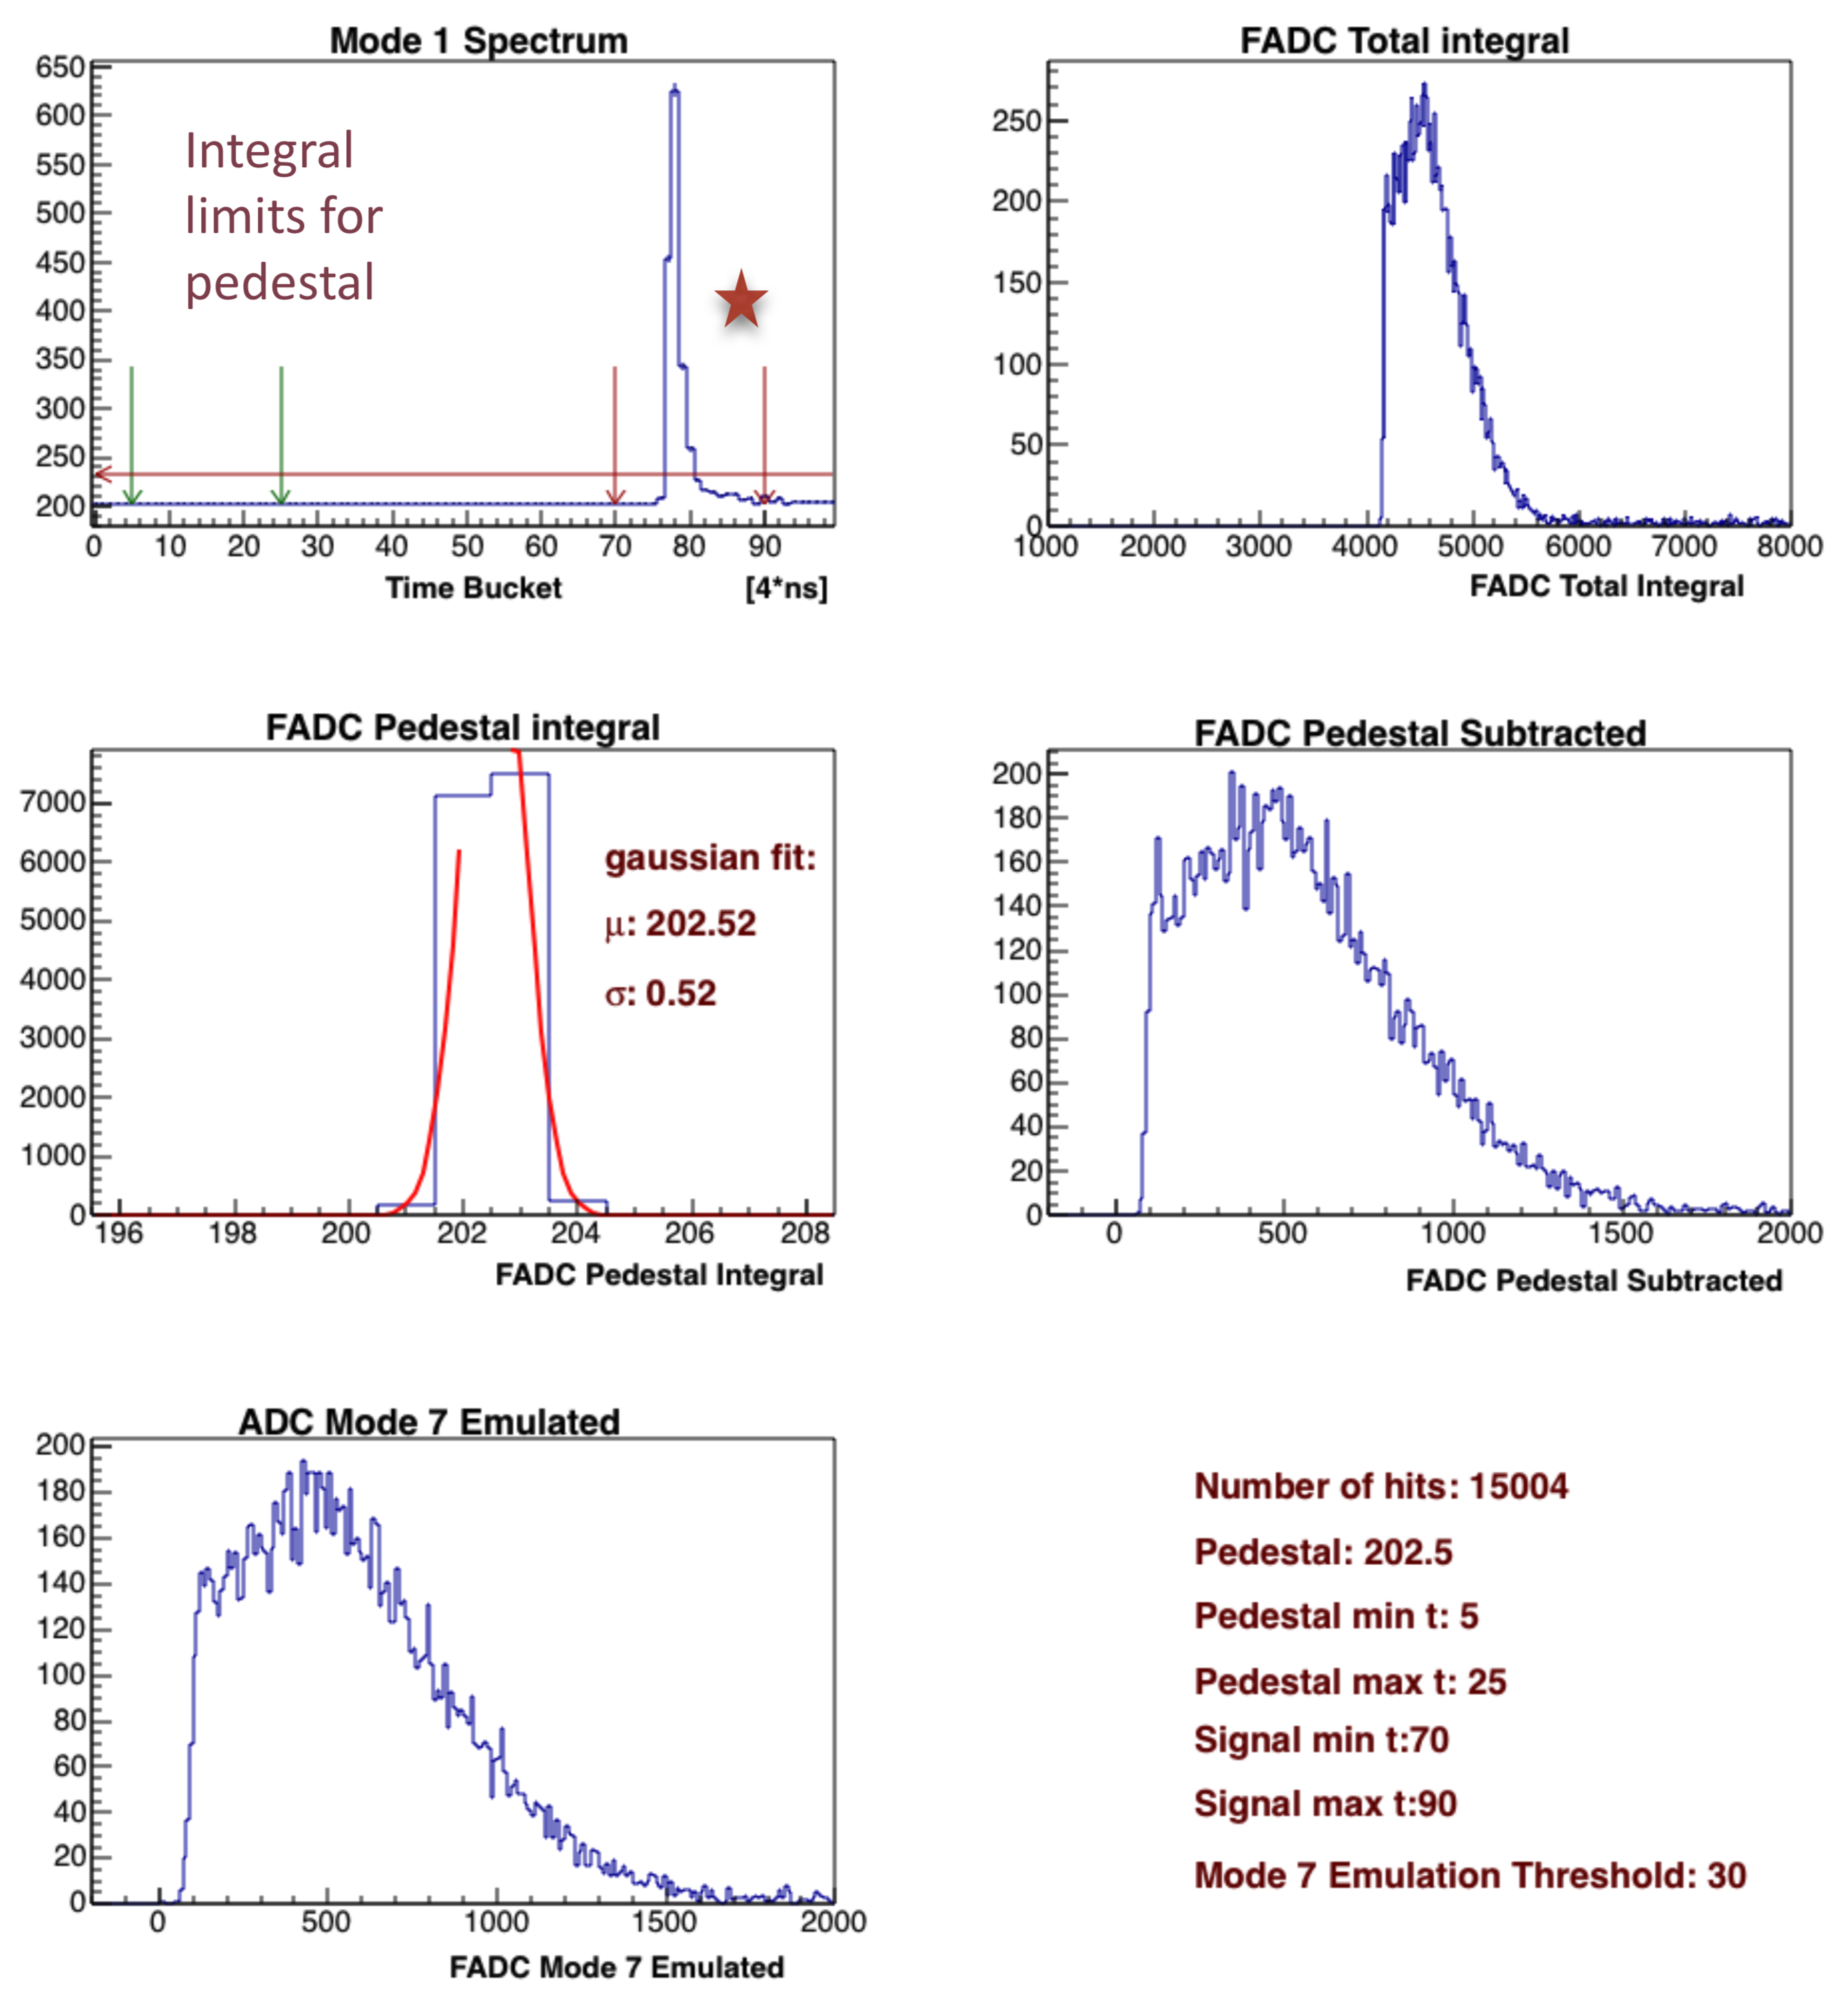
\includegraphics[width=0.95\columnwidth,keepaspectratio]{img/readout.png}
%	\caption{The electronic scheme of the LTCC.}
%	\label{fig:readout}
%\end{figure}
